\documentclass[a4paper]{article}
\usepackage[printsolution=true]{exercises}
\usepackage{url}
\usepackage{background, hyperref}
\usepackage{tcolorbox}
\usepackage{lastpage}
\usepackage{fancyhdr}
\usepackage{xcolor}
\usepackage[sfdefault]{cabin}
\usepackage{graphicx}
\usepackage[T1]{fontenc}
\usepackage[backend=bibtex,style=authoryear,natbib=true]{biblatex}
\bibliography{howeetal18.bib}
%\bibliographystyle{besjournals}
\setlength\parindent{0pt}

\pagestyle{fancy}
\fancyhead[L,C,R]{}
\fancyfoot[L]{\small CTDS workshop, Univ. of St Andrews}
\fancyfoot[R]{\small Practical 2 - duiker detections}
\fancyfoot[C]{\small \thepage\ of \pageref{LastPage}}
\renewcommand{\headrulewidth}{0pt}
\renewcommand{\footrulewidth}{1pt}

\newif\iffirstpage
\firstpagetrue
\backgroundsetup{contents={%
 			\iffirstpage
				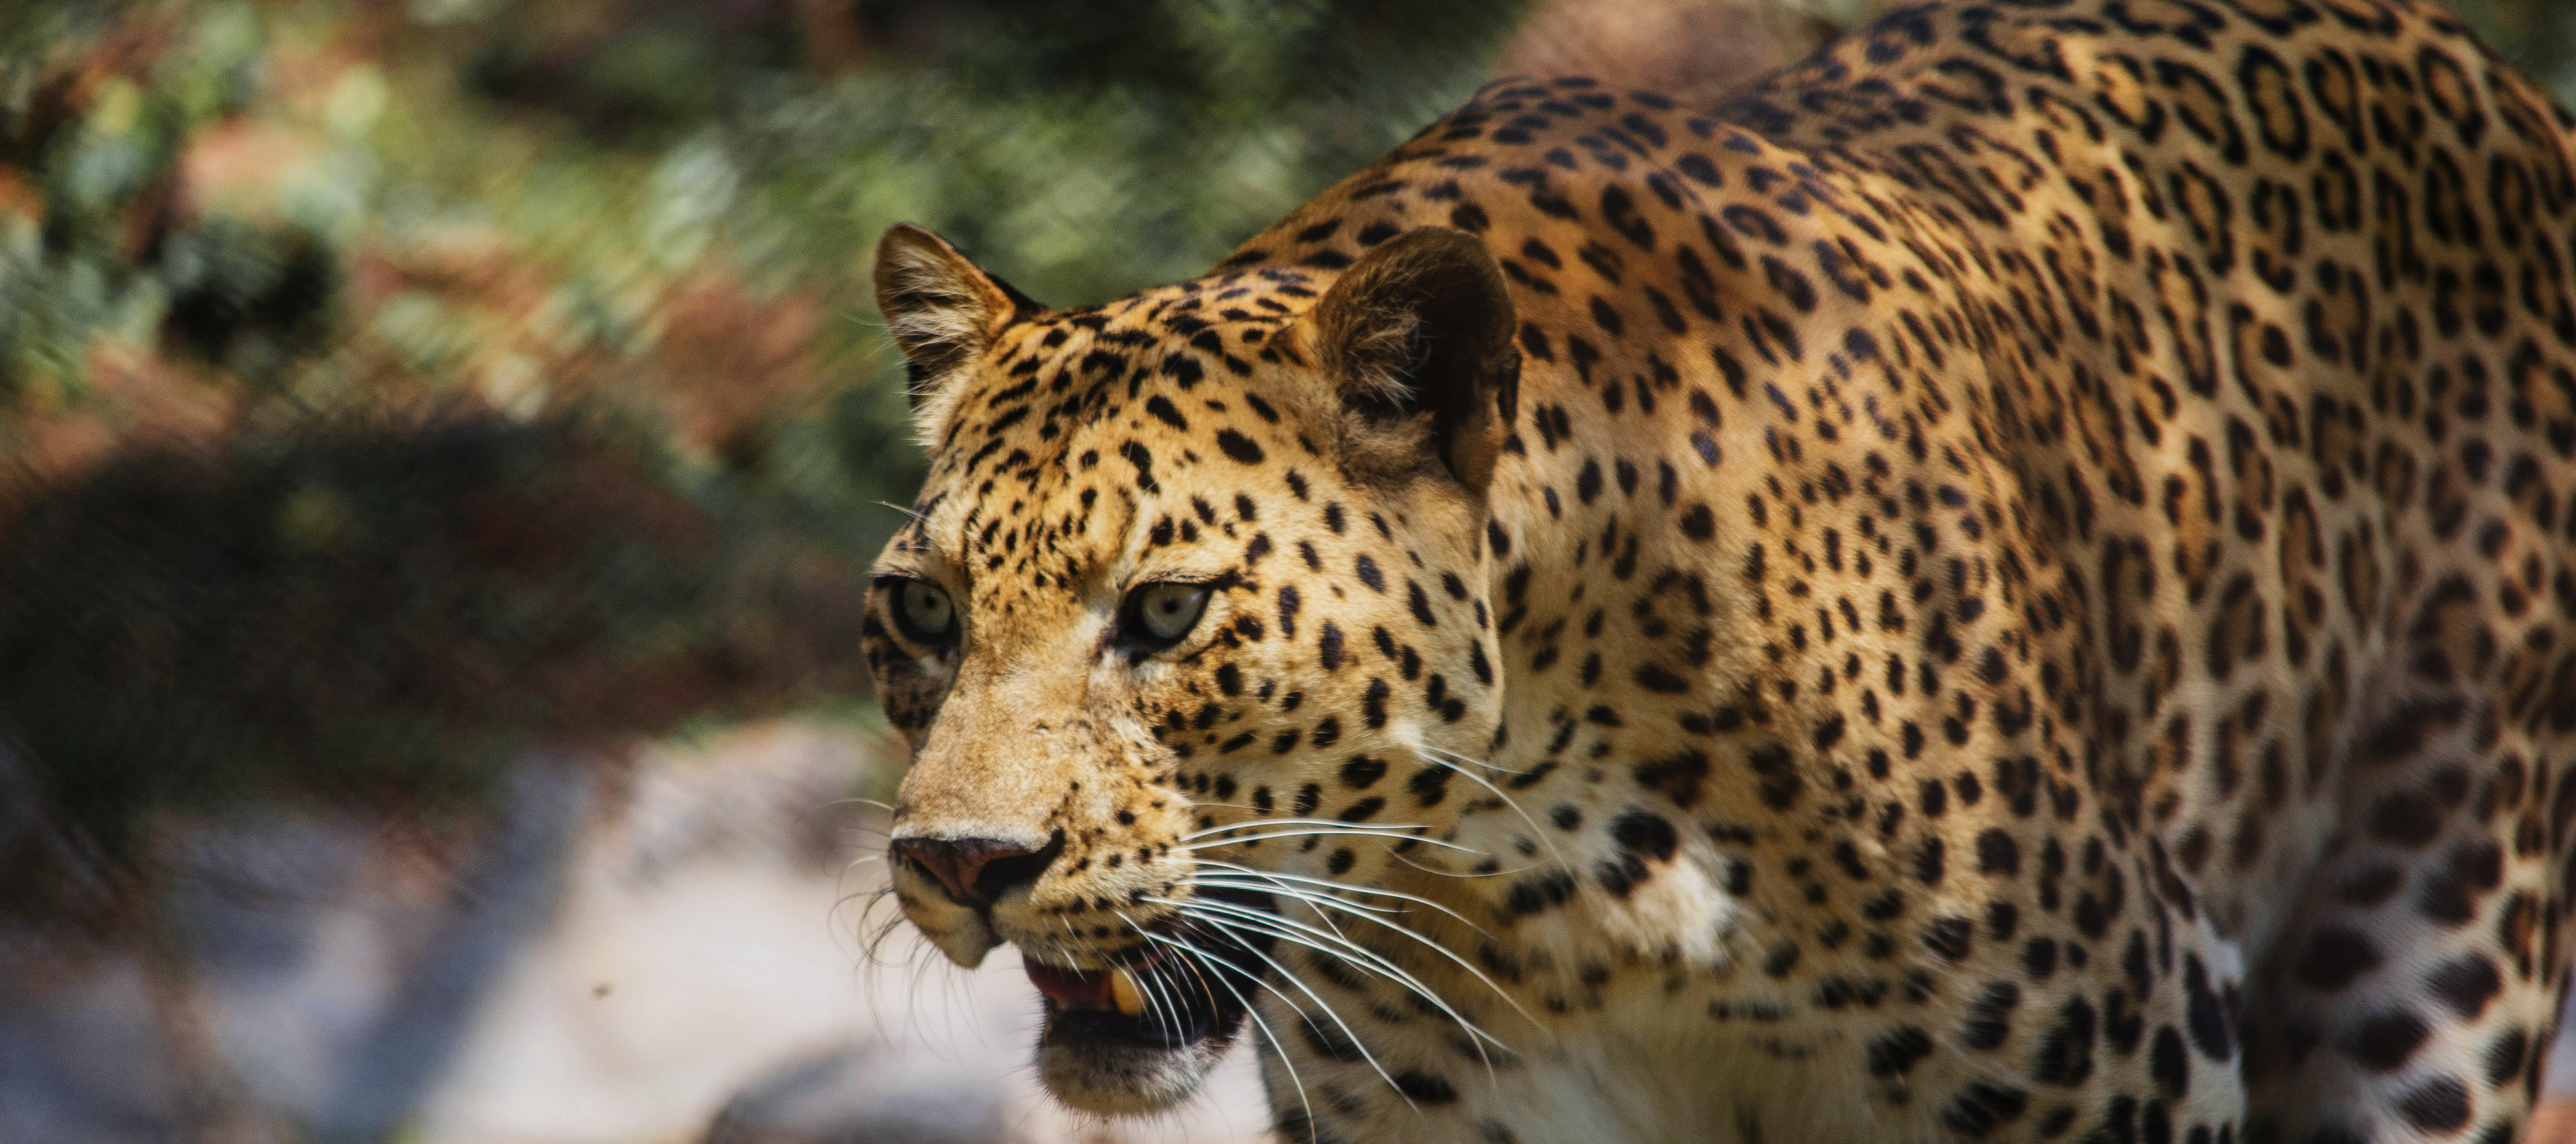
\includegraphics[width=\textwidth]{jaguar1.jpg}%
				\global\firstpagefalse
				\fi
			},
			scale=1,placement=top,opacity=0.6,position=current page.north, vshift=-1cm
}

\begin{document}
%% don't mess with blank lines here in the title.
\phantom{a}

\bigskip

{\Large Camera trap distance sampling workshop}

{\large 21-25 March 2022}

\begin{flushright}
\tiny{Source: \url{https://unsplash.com/@satyadeep_d}}
\end{flushright}

\ifsolutionthenelse{%
{\Large \color{blue}Solution \\}
{\color{blue}\rule{\linewidth}{0.5mm}}
}%
{%
}

A distance sampling approach to the analysis of camera trapping data offers the potential advantage that individual animal identification is not required. However, accurate animal-to-camera detection distances are required. This requires calibration prior to the survey with images of objects of known size taken at known distances from the camera. See details in \citep{howeetal} for description of the field work and data analysis. Here we present analysis of data from \citep{howeetal} using Distance for Windows \citep{Thomas2010}. 

\section{Data input}

A data set for recording of detections during daytime are in the Distance for Windows project associated with this practical.  The data themselves are in an online repository \citep{dryad}

\emph{Open the DistWin project \texttt{DuikerDaytime.zip} that you have downloaded to your computer.}

Glance through the data window, noting one camera station (E4) had no detections.

\subsection{Distance recording: binning and truncation}
Distance bins are set to be narrow out to 8m, then increasing in width to the maximum detection distance of 21m.

As described in \cite{howeetal}
\begin{quotation}
a paucity of observations between 1 and 2 m but not between 2 and 3 m, so we left-truncated at 2 m. Fitted detection functions and probability density functions were heavy-tailed when distances >15 m were included, so we right truncated at 15 m.
\end{quotation}

\section{Detection function modelling}
Candidate models include 
\begin{itemize}
	\item half normal key with 0 and 1 Hermite polynomial adjustment
	\item uniform key with 1 and 2 cosine adjustments and 
	\item hazard rate key with 0, 1 and 2 cosine adjustments. 
\end{itemize}
 
 Note, rather than allow Distance for Windows to perform within-key function model selection of adjustment terms, we explicitly fit each adjustment term model.

\section{Model criticism}

Having fitted the seven models described above, examine the output of each model to assess fit.  Also look at the \emph{Results Browser} for AIC metrics.

\ifsolutionthenelse{%
	\begin{tcolorbox}[colback=green!5!white, colframe=green!60!black, title=Results browser for fitted models]
{\small
\begin{tabular}{lrrrrrrr}
Name              & params & $\Delta$AIC & D     & D LCL & D UCL & D CV & GOF $\chi^2$ p \\
\hline
hn herm 0 left 2  & 1        & 131.45    & 15.44 & 8.91  & 26.77 & 0.27 & 0.00      \\
hn herm 1 left 2  & 2        & 95.44     & 14.37 & 8.28  & 24.92 & 0.27 & 0.00      \\
unif cos 1 left 2 & 1        & 78.81     & 13.18 & 7.60  & 22.84 & 0.27 & 0.00      \\
unif cos 2 left 2 & 2        & 73.09     & 13.92 & 8.02  & 24.14 & 0.27 & 0.00      \\
haz cos 0 left 2  & 2        & 19.00     & 10.55 & 6.09  & 18.30 & 0.27 & 0.00      \\
haz cos 1 left 2  & 3        & 20.67     & 11.09 & 6.36  & 19.34 & 0.27 & 0.00      \\
haz cos 2 left 2  & 4        & 0.00      & 11.30 & 6.43  & 19.88 & 0.28 & 0.00     
\end{tabular}
}
\end{tcolorbox}
}
{
}

\section{Questions about this analysis}

\begin{itemize}
\item What might be justification for left truncation?
\ifsolutionthenelse{%
	\begin{tcolorbox}[colback=green!5!white, colframe=green!60!black, title=Left truncation]
	If animals close to the detector respond, detections (or lack thereof) may not be representative of the detection process. Similarly, if the vertical field of view of the detectors do not detect animals short in stature close to the detector, then left truncation might be justified. 
\end{tcolorbox}
}
{
}
	\begin{itemize}
		\item What are the dangers of such truncation?
\ifsolutionthenelse{%
	\begin{tcolorbox}[colback=green!5!white, colframe=green!60!black, title=Left truncation challenges]
		The truncation distance is subjective.  Remember it is detections at small distances that are fundamental to estimating $\hat{h}(0)$: slope of the PDF at distance 0.  This estimate is estimated via extrapolation when left truncation is used.
		\end{tcolorbox}
}
{
}
	\end{itemize}
\item Initial assessment of fit of models?
\ifsolutionthenelse{%
	\begin{tcolorbox}[colback=green!5!white, colframe=green!60!black, title=Model fit]
Note the P-values for all goodness of fit tests is effectively zero, meaning none of the models fit the data because of overdispersion.
		\end{tcolorbox}
}
{
}
\item What is your preliminary model choice?
\ifsolutionthenelse{%
	\begin{tcolorbox}[colback=green!5!white, colframe=green!60!black, title=Model selection]
Using traditional AIC for model selection, we would conclude that the hazard rate model without adjustments is the best of the candidate models for these data.
		\end{tcolorbox}
}
{
}\end{itemize}

\printbibliography

\end{document}